\documentclass[10pt]{article} % Font size - 10pt, 11pt or 12pt

\usepackage[hmargin=1.25cm, vmargin=1.5cm]{geometry} % Document margins

\usepackage{graphicx}
\usepackage{amsmath}
\usepackage{marvosym} % Required for symbols in the colored box
\usepackage{ifsym} % Required for symbols in the colored box

\usepackage[usenames,dvipsnames]{xcolor} % Allows the definition of hex colors

% Fonts and tweaks for XeLaTeX
\usepackage{fontspec,xltxtra,xunicode}
\defaultfontfeatures{Mapping=tex-text}
%\setmonofont[Scale=MatchLowercase]{Andale Mono}

% Colors for links, text and headings
\usepackage{hyperref}
\definecolor{linkcolor}{HTML}{506266} % Blue-gray color for links
\definecolor{shade}{HTML}{F5DD9D} % Peach color for the contact information box
\definecolor{text1}{HTML}{2b2b2b} % Main document font color, off-black
\definecolor{headings}{HTML}{701112} % Dark red color for headings
% Other color palettes: shade=B9D7D9 and linkcolor=A40000; shade=D4D7FE and linkcolor=FF0080

\hypersetup{colorlinks,breaklinks, urlcolor=linkcolor, linkcolor=linkcolor} % Set up links and colors

\usepackage{fancyhdr}
\pagestyle{fancy}
\fancyhf{}
% Headers and footers can be added with the \lhead{} \rhead{} \lfoot{} \rfoot{} commands
% Example footer:
%\rfoot{\color{headings} {\sffamily Last update: \today}. Typeset with Xe\LaTeX}

\renewcommand{\headrulewidth}{0pt} % Get rid of the default rule in the header

\usepackage{titlesec} % Allows creating custom \section's

\allowdisplaybreaks

% Format of the section titles
\titleformat{\section}{\color{headings}
\scshape\Large\raggedright}{}{0em}{}[\color{black}\titlerule]

\title{Classical Mechanics Assignment 7}
\author{Elliott Capek}
\titlespacing{\section}{0pt}{0pt}{5pt} % Spacing around titles

\begin{document}

\maketitle{}

\section{Problem One}
\textbf{Consider a simple plane pendulum consisting of a mass m attached to a string of length l. After the pendulum is set into motion, the length of the string is shortened at a constant rate:}
\begin{equation}
  \frac{dl}{dt} = −\alpha
\end{equation}

\textbf{The suspension point remains fixed. Compute the Lagrangian and Hamiltonian functions. Compare the Hamiltonian and the total energy, and discuss the conservation of energy for the system.}

\section{Problem One: Shrinking Pendulum Hamiltonian}


\begin{align*}
  x &= \ell\sin\theta\\
  y &= -\ell\cos\theta\\

  \dot{x} &= -\alpha\sin\theta + \ell\cos\theta\dot{\theta}\\
  \dot{y} &= \alpha\cos\theta + \ell\sin\theta\dot{\theta}\\
  \vspace{1cm}\\
  T &= \frac{1}{2}mv^2 = \frac{1}{2}m\left(\alpha^2+\ell^2\dot{\theta}^2\right)\\
  U &= mgy = -mg\ell\cos\theta\\
  \mathcal{L} &= \frac{1}{2}m\left(\alpha^2+\ell^2\dot{\theta}^2\right) + mg\ell\cos\theta\\
\end{align*}


  \dot{x} &= \dot{\ell}\sin\theta + \ell\cos\theta\dot{\theta}\\
  \dot{y} &= -\dot{\ell}\cos\theta + \ell\sin\theta\dot{\theta}\\
  \vspace{1cm}\\
  T &= \frac{1}{2}m\left(\dot{\ell}^2 + \ell^2\dot{\theta}^2\right)\\
  U &= -mg\ell\cos\theta\\
  \mathcal{L} &= \frac{1}{2}m\left(\dot{\ell}^2 + \ell^2\dot{\theta}^2\right) + mg\ell\cos\theta\\
  \vspace{1cm}\\
  p_{\theta} &= m\ell^2\dot{\theta}\\
  p_{\ell} &= m\dot{\ell}\\
  \mathcal{H} &= p_{\theta}\dot{\theta} + p_{\ell}\dot{\ell} - \mathcal{L} = m\ell^2\dot{\theta}^2 + m\dot{\ell}^2 - \frac{1}{2}m\left(\dot{\ell}^2 + \ell^2\dot{\theta}^2\right) - mg\ell\cos\theta\\
  &= \frac{1}{2}m\left(\alpha^2 + \ell^2\dot{\theta}^2\right) - mg\ell\cos\theta\\
  \vspace{1cm}\\
  T + U &= \frac{1}{2}m\left(\alpha^2 + \ell^2\dot{\theta}^2\right) - mg\ell\cos\theta\\
\end{align*}

As we can see, the Hamiltonian and the total energy for this system are identical. Because the Lagrangian for this system has no time-dependence, we know that $\mathcal{H}$ must be conserved, and thus total energy is conserved.\\

This problem was a basic tour of how to set up problems using the Hamiltonian. We didn't solve it to completion, but the answer could have been found by deriving $\mathcal{H}$ with respect to momentum and the velocities. It took me a second to figure out this problem, since I wasn't considering that there are actually two generalized coordinates in this problem - $\theta$ and $l$. Once I figured this out, the problem became much easier.\\

\section{Problem Two: 3D Pendulum Hamiltonian}

\textbf{A spherical pendulum consists of a bob of mass m attached to a weightless extension rod of length l. The end of the rod opposite the bob pivots freely (in all directions) about some fixed point. Set up the Hamiltonian function in spherical coordinates. (If $p_{\phi}=0$, the result is the same as that for the plane pendulum.) Combine the term that depends on $p_{\phi}$ with the ordinary potential energy to find the effective potential $V(\theta,p_{\phi})$. Sketch V as a function of $\theta$ for several values of $p_{\phi}$, including $p_{\phi}$ = 0. Discuss the features of the motion, pointing out the differences between $p_{\phi}=0$ and $p_{\phi} \neq 0$. Discuss the limiting case of the conical pendulum ($\theta = $constant) with reference to the V − $\theta$ diagram.}

\begin{align*}
  x &= \ell\cos\phi\sin\theta\\
  y &= \ell\sin\phi\sin\theta\\
  z &= \ell\cos\theta\\
  \dot{x} &=  -\ell\sin\phi\sin\theta\dot{\phi} + \ell\cos\phi\cos\theta\dot{\theta}\\
  \dot{y} &= \ell\cos\phi\sin\theta\dot{\phi} + \ell\sin\phi\cos\theta\dot{\theta}\\
  \dot{z} &= -\ell\sin\theta\dot{\theta}\\
  \vspace{1cm}\\
  T &= \frac{1}{2}m\left(\dot{x}^2+\dot{y}^2+\dot{z}^2\right)\\
  &= \frac{1}{2}m\ell^2\left(\sin^2\theta\dot{\phi}^2 + \dot{\theta}^2\right)\\
  U &= mgz = mg\ell\cos\theta\\
  \mathcal{L} &= \frac{1}{2}m\ell^2\left(\sin^2\theta\dot{\phi}^2 + \dot{\theta}^2\right) - mg\ell\cos\theta\\
  \vspace{1cm}\\
  P_{\theta} &= \frac{d\mathcal{L}}{d\dot{\theta}} = m\ell^2\dot{\theta}\\
  P_{\phi} &= \frac{d\mathcal{L}}{d\dot{\phi}} = m\ell^2\sin^2(\theta)\dot{\phi}\\
  \vspace{1cm}\\
  \vspace{1cm}\\
  \mathcal{H} &= P_{\theta}\dot{\theta} + P_{\phi}\dot{\phi} - \mathcal{L}\\
  &= \frac{1}{2}m\ell^2\left(\sin^2\theta\dot{\phi}^2 + \dot{\theta}^2\right) + mg\ell\cos\theta\\
  &= \frac{1}{2}m\ell^2\left(\sin^2\theta\dot{\phi}^2 + \frac{P_{\theta}^2}{m^2\ell^4}\right) + mg\ell\cos\theta\\

    V_{eff}(\theta, P_{\phi}) &=
\end{align*}


\begin{figure}[h]
\caption{Plot of effective potential based on $p_{\phi}$ and gravity potential. Angular momentum linearly adds to the sinusoidal gravity potential.}
\centering
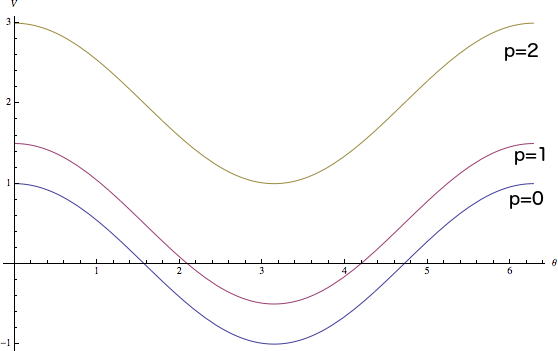
\includegraphics[width=0.5\textwidth]{../v-plot_legend.png}
\end{figure}

\section{Problem Three}
\textbf{A bead of mass m is threaded on a frictionless wire that is bent into a helix with cylindrical polar coordinates (ρ, ϕ, z) satisfying z = cϕ and ρ = R with c and R constants. The z axis points vertically up and gravity vertically down. Using ϕ as your generalized coordinate, write down the kinetic and potential energies and the Hamiltonian H as a function of ϕ and its conjugate momentum p. Write down Hamilton’s equations and solve for φ!!and hence !z!. Explain your result in terms of Newtonian mechanics and discuss the special case that R = 0.}

\end{document}


\begin{align*}
  x &= \ell\sin\phi\cos\theta\\
  y &= \ell\sin\phi\sin\theta\\
  \dot{x} &= \ell\cos\phi\cos\theta\dot{\phi} - \ell\sin\phi\sin\theta\dot{\theta}\\
  \dot{y} &= \ell\cos\phi\sin\theta\dot{\phi} + \ell\sin\phi\cos\theta\dot{\theta}\\
  \vspace{1cm}\\
  T &= \frac{1}{2}m\left(\ell^2\cos^2\phi\dot{\phi}^2 + \ell^2\sin^2\phi\dot{\theta}^2\right)\\
  U &= mgz = mg\ell\cos\theta\\
  \mathcal{L} &= \frac{1}{2}m\left(\ell^2\cos^2\phi\dot{\phi}^2 + \ell^2\sin^2\phi\dot{\theta}^2\right) - mg\ell\cos\theta\\
  \vspace{1cm}\\
  \mathcal{H} &= p_{\theta}\dot{\theta} + p_{\phi}\dot{\phi} - \mathcal{L}\\
  &= m\ell\sin\phi\dot{\theta}^2 + m\ell\cos\phi\dot{\phi}^2 - \frac{1}{2}m\left(\ell^2\cos^2\phi\dot{\phi}^2 + \ell^2\sin^2\phi\dot{\theta}^2\right) + mg\ell\cos\theta\\
  &= \frac{1}{2}m\left(\ell^2\cos^2\phi\dot{\phi}^2 + \ell^2\sin^2\phi\dot{\theta}^2\right) + mg\ell\cos\theta\\
  &= \frac{p_{\theta}^2}{2m} + \frac{p_{\phi}^2}{2m} + mg\ell\cos\theta\\
  V(\theta,p_{\phi}) &= \frac{p_{\phi}^2}{2m} + mg\ell\cos\theta = \frac{1}{2}m\ell^2\cos^2\phi\dot{\phi}^2 + mg\ell\cos\theta\\
\end{align*}
